\documentclass[preprint,numbers,10pt]{sigplanconf}

\usepackage{hyperref}
\usepackage{graphicx}
\usepackage{xcolor}
\newcommand\comment[1]{\textcolor{blue}{#1}}

\begin{document}

\title{Language Workbench Challenge 2016: the Jetbrains MetaProgramming System}

\authorinfo{Eugen Schindler}{}{eugenschindler@gmail.com}
\authorinfo{Klemens Schindler}{}{klemensschindler@gmail.com}
\authorinfo{Federico Tomassetti}{Independent}{federico@tomassetti.me}
\authorinfo{Markus V\"{o}elter}{}{voelter@gmail.com}
\authorinfo{Kolja Dummann}{}{k.dummann@gmail.com}
\authorinfo{Remi Bosman}{}{remi.bosman@gmail.com}
\authorinfo{Ana Maria \c{S}ut\^{i}i}{}{farcasia@gmail.com}

\maketitle

%%%%%%%%%%%%%%%%%%%%%%%%%%%%%%%%%%%%%%%%%%%%%%%%%%%%%%%%%%%%%%%%%%%%%%%%%%%%%%%
%
% Introduction
%
%%%%%%%%%%%%%%%%%%%%%%%%%%%%%%%%%%%%%%%%%%%%%%%%%%%%%%%%%%%%%%%%%%%%%%%%%%%%%%%

\section{Introduction}

In this paper, we are going to discuss how the JetBrains MetaProgramming System can be used to address the problems presented in the Language Workbench Challenge 2016 (LWC'16).

The Jetbrains MetaProgramming System (MPS) is a mature Language Workbench based on projectional editing. While other Language Workbenches are based on projectional editing (the Whole Platform \cite{solmi2005whole}, MetaEdit+ \cite{Tolvanen2006}, Intentional Domain Workbench \cite{Simonyi2006}) MPS is arguably the most mature, with a growing user base.

We believe that one key feature to make MPS successful is its flexibility. By using a powerful and flexible Language Workbench such MPS we, as Language Engineers, can provide languages and corresponding tools that support a significant overhaul of the processes of an organization. It is frequently the case that such processes involve very different kinds of users with very different backgrounds, experiences, and needs. Therefore a complete solution could potentially encompass different aspects of the internal processes, providing different views and a variety of tools such as simulators, debuggers, code-generators, and more.

The ability to support different notations, to process models in different ways, to perform validation and support testing: all these features and others are necessary to build solutions as complete as demanded in real-life scenarios.

Considering the comparison of Language Workbenches features presented in \cite{erdweg2015evaluating} we can see that MPS is among the most complete Language Workbenches. Other tools with a comparable level of completeness are \emph{MetaEdit+} and the \emph{Whole Platform}. While \emph{Xtext} \cite{Eysholdt2010} has a strong support in many areas it is strictly confined to the textual notation and this limitation sets it apart from multi-notation Language Workbenches such as MPS.

With respect to the feature model presented in \cite{erdweg2015evaluating} the only features missing in MPS are \emph{Free-form editing} and \emph{Live translation}.

\subsection{Jetbrains MPS in previous challenges}

TODO: Summarize results of MPS in previous challenges

\subsection{Problems presented in the LWC'16}

The problems identified for the LWC'16 permit to evaluate very different aspects of a Language Workbench. By addressing all three of them we aim to offer a complete picture of the potentialities (and possibly the limitations) offered by MPS.

The first problem is regarding \textbf{Notation}. By addressing this problem we aim to demonstrate how MPS can support several, very different notations. Notations are particularly relevant because they are the most visible aspect of languages. In many cases, Language Workbenches are used to create Domain Specific Languages. Such languages are intended to appeal a specific category of subjects. This category could be familiar with specific notations, not necessarily textual. Being able to support the notations of preference of the target audience can be a key element to winning users support. 

The second problem considers \textbf{Evolution and Reuse}. These are characteristics which are absolutely crucial for the maintenance of a solution in the long run. Any mature engineering approach should consider the whole lifecycle of the proposed solution. The evolution is particularly important for languages because they are tools used to represent knowledge, probably the most valuable asset for many companies. By being able to evolve languages we can preserve the investment done in building models using those languages. Reuse is another key element because it permits to significantly reduce the cost of developing complex solutions. For example, several projects based on MPS benefit from reusing languages provided as part of the \emph{mbeddr platform} \footnote{See \url{http://mbeddr.com/platform.html}}.

Finally, the third problem is about \textbf{Editing}. This aspect is particularly relevant for projectional editors because they usually require users to part from the traditional textual editing experience. This transition requires significant training and it can be a cause of resistance. By improving the editing experience we can reduce this risk. While the usability of the MPS editors have been previously deemed positive by users \cite{Voelter2014} we believe is still an aspect which needs to be emphasized. By addressing this particular problem we aim to prove the progresses of MPS in this area and highlight possible necessary improvements still needed.

\subsection{Structure of the paper}

In the rest of the paper we are going to present our proposed solutions to the three different problems (\emph{Notation, Evolution and Reuse, and Editing}). For each problem we will start by describing the assumptions, then we will discuss the implementation, separately for each point, and after that we will analyze each problem according to this schema: Variants, Usability, Impact, Composability, Limitations, Uses and examples, Effort (best-effort), Other comments, Artifact.

Finally, we will draw our conclusions.

%%%%%%%%%%%%%%%%%%%%%%%%%%%%%%%%%%%%%%%%%%%%%%%%%%%%%%%%%%%%%%%%%%%%%%%%%%%%%%%
%
% Notation Section
%
%%%%%%%%%%%%%%%%%%%%%%%%%%%%%%%%%%%%%%%%%%%%%%%%%%%%%%%%%%%%%%%%%%%%%%%%%%%%%%%

\section{Addressing the Notation Problem}

\subsection{Assumptions}

\subsection{Implementation}
The implementation for this challenge is located in a repository on github \footnote{https://github.com/mps-lwc-16/mps-lwc-16}. To explore the implementation, please clone the repository and follow the instructions in the README.md.

Many of the challenge items can be demonstrated using examples from the \emph{mbeddr platform} \footnote{See \url{http://mbeddr.com/platform.html}}, so we have used examples from there whenever appropriate.

We have written models in the mbeddr documentation language to present the implementation. To open the documentation model for the implementation to this challenge, open the Notation model, as shown in Figure \ref{fig:opennotation}. The Notation chapter is divided into sections, each of which addresses one or more of the challenge items. Each of those items is discussed in detail in the subsections below.

\begin{figure}[p]
	\centering
	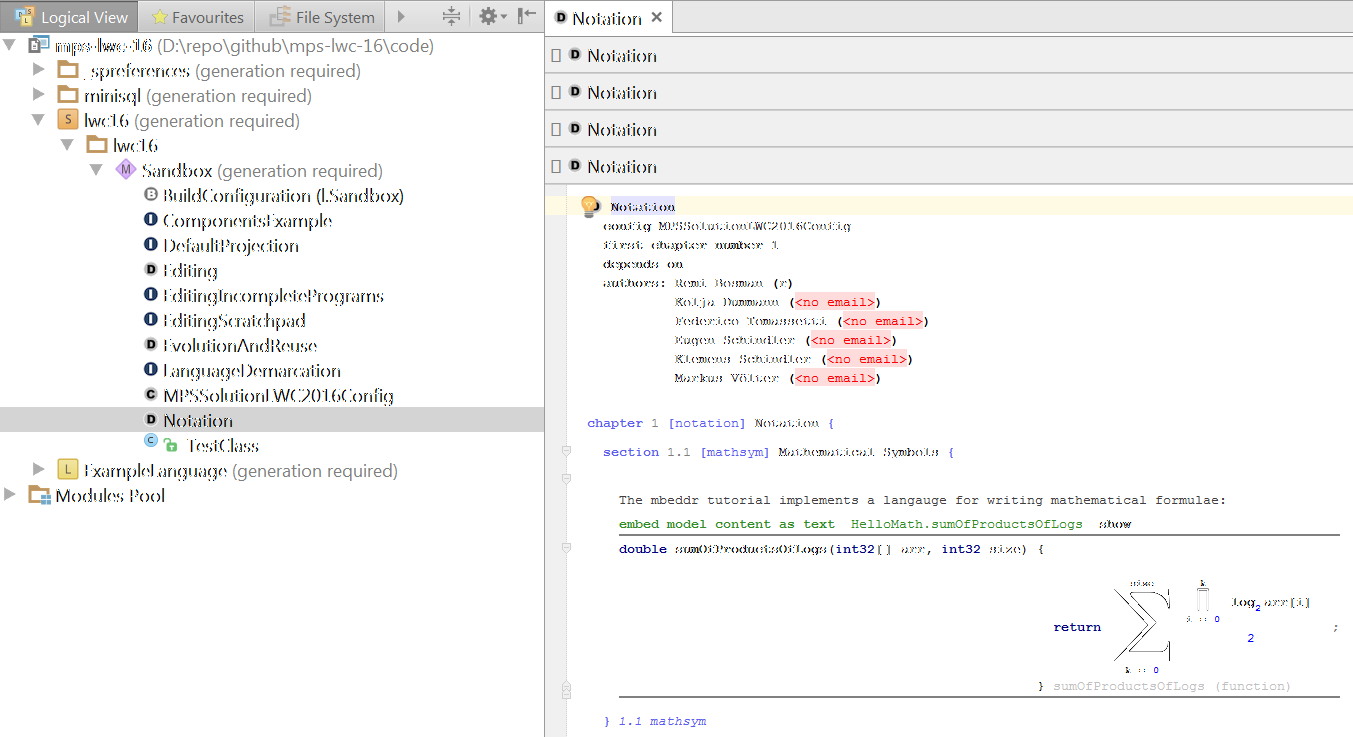
\includegraphics[width=0.50\textwidth]{screens/OpenNotation.png}
	\caption{The documentation model for the Notation challenge}
	\label{fig:opennotation}
\end{figure}

\subsubsection{Support mathematical symbols, tabular notation, diagrammatic notations in addition to textual notation, and support switching between multiple alternative notations for the same language}
This subsection addresses four of the challenge items at once:
\begin{itemize}
	\item Support mathematical symbols in addition to textual notation: see Figure \ref{fig:mathnotation}.
	\item Support tabular notation in addition to textual notation
	\item Support diagrammatic notation in addition to textual notation
	\item Support alternative notations for the same language
\end{itemize}

\begin{figure}[p]
	\centering
	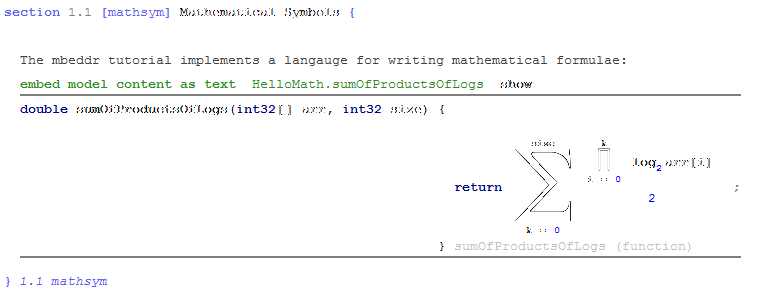
\includegraphics[width=0.50\textwidth]{screens/MathematicalNotation.png}
	\caption{The documentation model for the Notation challenge}
	\label{fig:mathnotation}
\end{figure}

\subsubsection{Generic metadata annotations: annotation of program elements without changing their core meaning}
\subsubsection{Optional hiding: hide parts of the code, without losing the content and while retaining editability}
\subsubsection{Computed properties: read only annotations that are automatically derived form the main program}
\subsubsection{Computed structures: structured, editable views}
\subsubsection{Skeleton editing: guide the user with syntactic templates with editable holes}
\subsubsection{Embedding code in prose: mix structured code with free text}
\subsubsection{Embedding blackboxes: allow program elements to be opaque non-textual elements}

\subsection{Variants}

\subsection{Usability}

\subsection{Impact}

\subsection{Composability}

\subsection{Limitations}

\subsection{Uses and examples}

\subsection{Effort (best-effort)}

\subsection{Other comments}

\subsection{Artifact}

%%%%%%%%%%%%%%%%%%%%%%%%%%%%%%%%%%%%%%%%%%%%%%%%%%%%%%%%%%%%%%%%%%%%%%%%%%%%%%%
%
% Evolution and Reuse Section
%
%%%%%%%%%%%%%%%%%%%%%%%%%%%%%%%%%%%%%%%%%%%%%%%%%%%%%%%%%%%%%%%%%%%%%%%%%%%%%%%

\section{Addressing the Evolution and Reuse Problem}

\subsection{Assumptions}

Our solutions are presented making references to the two main language families developed for MPS.
First of all we have the BaseLanguage, which is an implementation of Java built from Jetbrains and shipped with MPS. Several extensions are distributed with MPS, including extensions to support lambdas, manipulation of sequences, expressions to access MPS concepts and models, etc.
Another very popular family of languages is mbeddr. It is an implementation of the C language in MPS with support for variability, state machines, testing, documentation and more. In addition to the the mbeddr platform has been created. It is a collection of language extensions not specifically related to mbeddr or the C language. These extensions proved to be useful in were different contexts.

\subsection{Implementation}

\subsubsection{Language extension: modularly extend a language with new syntactic constructs}

In this section, we are going to describe the mbeddr language for state
machines with event-driven execution. The mbeddr state machines extends
the base language from MPS. This enables a seamless integration between
C code and state machine specifications.

State machines are a mathematical model of computation often used in embedded software
for describing discrete behaviour through state transitions. Its characterizing
ingredients are states, transitions and events. At any given time, a state
machine is in a state and it can be transitioned from one state to another.
A transition in a state machine is triggered by an event. These events
are usually provided by the environment, and, hence, the state machine
needs to have a way to interact with the environment. Besides events,
transitions can also have different guard expressions that need to hold when
the event arrives, for the transitions to be triggered.

We are now going to describe the extension of mbeddr with new syntactic notations for state machines.

In mbeddr, the state machine language is packaged in a language module and it
extends the base language of MPS. The \emph{StateMachine} concept extends
\emph{BaseConcept}, which means that the state machine is a program node,
as \emph{BaseConcept} is the concept from which all other concepts are derived.
The state machine language also implements the \emph{IModuleContent} interface,
which means that they can be top-level components in modules or can be inside of any
container that expects \emph{IModuleContent} children. Modules in mbeddr C
introduce basic program modularization, visibility control and namespaces \cite{voelter2013mbeddr}.

In the next paragraphs, we are going to present excerpts from a state machine for
judging flights. The state machine awards points for successful
takeoff and landing and for speed flown \cite{voelter2014generic}.

The state machine adds custom notation for specifying the state machine. The textual
form of the state machine can be seen in Figure \ref{fig:HFAT}. The figure depicts a hierarchical state machine
that computes the points for a flight.
In addition, because textual forms can live alongside graphical and tabular forms in MPS, 
the state machine can be viewed in table form and graphical form as well alongside the piece of C code
where it is used. Figure \ref{fig:HFATab} shows the same state machine for flight analyzes in tabular form.

\begin{figure}[ht!]
	\centering
	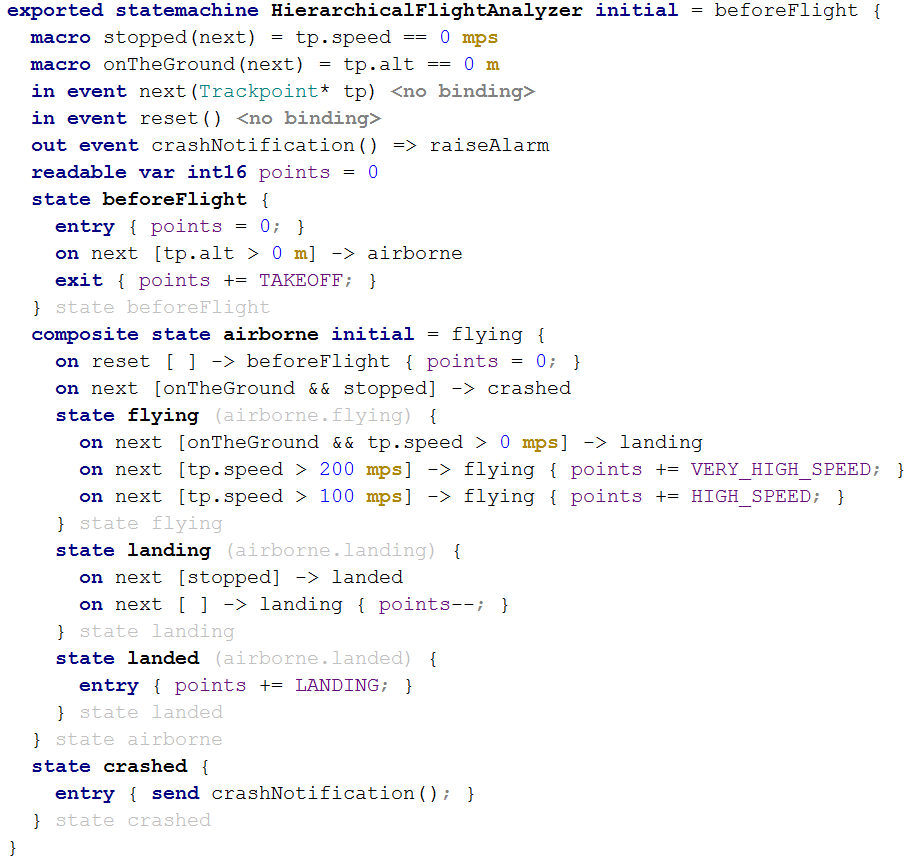
\includegraphics[scale=0.5]{screens/HierarchicalFlightAnalyzerT}
	\caption{Hierarchical flight analyzer state machine - textual notation}
	\label{fig:HFAT}
\end{figure}

\begin{figure*}[ht!]
	\centering
	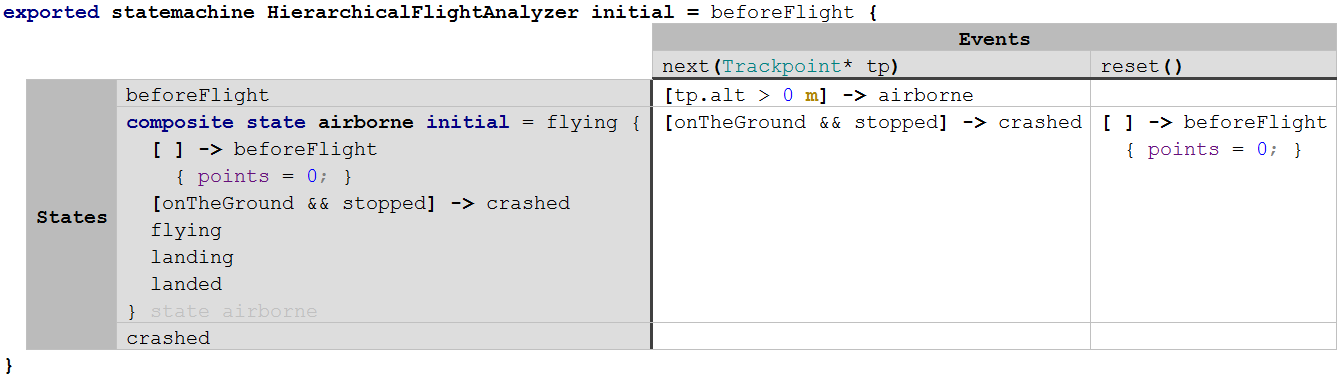
\includegraphics[scale=0.55]{screens/HierarchicalFlightAnalyzerTab}
	\caption{Hierarchical flight analyzer state machine - tabular notation}
	\label{fig:HFATab}
\end{figure*}

Moreover, the state machine itself embeds arbitrary code in the actions
and in the guards. The actions are statement lists and the guards are expressions.
For instance, look at the guards and actions in Figure \ref{fig:HFAT}; they contain mbeddr C expression.

\subsubsection{Language embedding: embed a separate language inside another}

We have implemented a simple toy language representing a subset of SQL. This language permits to define database schemas and simple SQL statements referring to such schemas.

Typically SQL is used in combinations with General Purpose Languages (GPLs): from the GPLs queries are generated by filling SQL templates with variable elements. The results of these queries are then possibly processed using GPL code.

In our example we implemented both embedding of C code into our MiniSQL and embedding of MiniSQL into C.
By embedding C code in MiniSQL we can define SQL statements with variable elements. For example we can refer to C variable containing an ID and refer to such ID in our SQL statement. In this way we can vary the value of the variable to obtain parametric SQL queries. We can then treat execute such queries using libraries such as those based on ODBC\footnote{See \url{https://en.wikipedia.org/wiki/Open_Database_Connectivity}}. It is important to notice that the MiniSQL embedded in C can be still edited with proper support regarding validation and auto-completion. It is not \"just a string\".
This technique is illustrated in \ref{fig:sqlembedding}.

\begin{figure}[p]
	\centering
	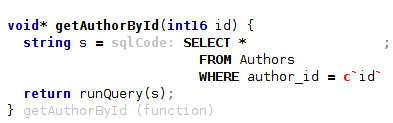
\includegraphics[width=0.50\textwidth]{screens/minisql_embedded.png}
	\caption{Embedding SQL code into C code and viceversa}
	\label{fig:sqlembedding}
\end{figure}

To demonstrate the flexibility of this approach we have also embedded our MiniSQL into the BaseLanguage, which is basically an implementation of Java in MPS. You can see it in \ref{fig:sqlembeddingjava}. Two separate extensions permit to embed the same language into different hosts (C and Java). For further explanations on this approach refer to \cite{Tomassetti2013}.

\begin{figure}[p]
	\centering
	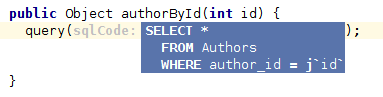
\includegraphics[width=0.50\textwidth]{screens/minisql_embedded_java.png}
	\caption{Embedding SQL code into Java code and viceversa}
	\label{fig:sqlembeddingjava}
\end{figure}

\subsubsection{Extension composition: combine independently developed extensions}



\subsubsection{Beyond grammar restrictions: disallow constructs in certain scopes, without modeling this in the (abstract) syntax}
\subsubsection{Syntax migration: support migrating programs when concrete syntax changes}
\subsubsection{Structure migration: support migrating programs when abstract syntax changes}

\subsection{Variants}

\subsection{Usability}

\subsection{Impact}

\subsection{Composability}

\subsection{Limitations}

\subsection{Uses and examples}

\subsection{Effort (best-effort)}

\subsection{Other comments}

\subsection{Artifact}

%%%%%%%%%%%%%%%%%%%%%%%%%%%%%%%%%%%%%%%%%%%%%%%%%%%%%%%%%%%%%%%%%%%%%%%%%%%%%%%
%
% Editing Section
%
%%%%%%%%%%%%%%%%%%%%%%%%%%%%%%%%%%%%%%%%%%%%%%%%%%%%%%%%%%%%%%%%%%%%%%%%%%%%%%%

\section{Addressing the Editing Problem}

\subsection{Assumptions}

\subsection{Implementation}

\subsubsection{Editing incomplete programs: support for syntactically malformed programs}
\subsubsection{Referencing missing items: support referencing items that have not been defined}
\subsubsection{Structure agnostic copy-paste: copy-paste works across syntax boundaries}
\subsubsection{Restructuring: changing syntactic structure without typing the complete expression again.}
\subsubsection{Language demarcation: show how a combination multiple languages in one program are disambiguated}
\subsubsection{Delayed decisions: show when the syntactic category of an expression is determined}
\subsubsection{End-user defined formatting: show if and how user can change the visual appearance of the program}
\subsubsection{Specification of default formatting: support for pretty printing}
\subsubsection{Formatting preservation: how is formatting preserved when the code is automatically restructured}

\subsection{Variants}

\subsection{Usability}

\subsection{Impact}

\subsection{Composability}

\subsection{Limitations}

\subsection{Uses and examples}

\subsection{Effort (best-effort)}

\subsection{Other comments}

\subsection{Artifact}

%%%%%%%%%%%%%%%%%%%%%%%%%%%%%%%%%%%%%%%%%%%%%%%%%%%%%%%%%%%%%%%%%%%%%%%%%%%%%%%
%
% Conclusions
%
%%%%%%%%%%%%%%%%%%%%%%%%%%%%%%%%%%%%%%%%%%%%%%%%%%%%%%%%%%%%%%%%%%%%%%%%%%%%%%%

\section{Conclusions}

The JetBrains MetaProgramming System has significantly evolved during the years. Nowadays it is a powerful and flexible tool that can be used to address most of the Language Engineering challenges that have been brought forward in the LWC 2016.

\textbf{Notation}
\textbf{Evolution and Reuse}
\textbf{Editing}

%% We are using the command `bibtex' from within the directory `build', thus we need
%% to go back from this directory and look for the bibliography file.
\bibliographystyle{plain}
\bibliography{../LWC2016}

\end{document}
